\documentclass[14pt, a4paper]{extarticle}
\usepackage{GOST}
\usepackage{array}
\usepackage{verbatim}
\usepackage[detect-all]{siunitx}
\usepackage{amsmath}
\usepackage{amssymb}
\usepackage[utf8]{inputenc}
\usepackage{hyperref}

\usepackage{ifthen}


\usepackage{tempora}



\makeatletter
\renewcommand\@biblabel[1]{#1.}
\makeatother

% Для листинга кода:
\usepackage{listings}
\lstset{ %
	language=c++,                 % выбор языка для подсветки (здесь это С)
	basicstyle=\small\sffamily, % размер и начертание шрифта для подсветки кода
	numbers=left,               % где поставить нумерацию строк (слева\справа)
	numberstyle=\tiny,           % размер шрифта для номеров строк
	stepnumber=1,                   % размер шага между двумя номерами строк
	numbersep=5pt,                % как далеко отстоят номера строк от подсвечиваемого кода
	showspaces=false,            % показывать или нет пробелы специальными отступами
	showstringspaces=false,      % показывать или нет пробелы в строках
	showtabs=false,             % показывать или нет табуляцию в строках
	frame=single,              % рисовать рамку вокруг кода
	tabsize=2,                 % размер табуляции по умолчанию равен 2 пробелам
	captionpos=t,              % позиция заголовка вверху [t] или внизу [b] 
	breaklines=true,           % автоматически переносить строки (да\нет)
	breakatwhitespace=false, % переносить строки только если есть пробел
	escapeinside={\#*}{*)}   % если нужно добавить комментарии в коде
}


%для графиков
\usepackage{pgfplots}
\usepackage{filecontents}
\usetikzlibrary{datavisualization}
\usetikzlibrary{datavisualization.formats.functions}

\begin{document}
	
	\begin{table}[ht]
		\centering
		\begin{tabular}{|c|p{400pt}|} 
			\hline
			\begin{tabular}[c]{@{}c@{}} 
\includegraphics[scale=1]{source/baum.jpg} \\\end{tabular} &
			\footnotesize\begin{tabular}[c]{@{}c@{}}\textbf{Министерство~науки~и~высшего~образования~Российской~Федерации}\\\textbf{Федеральное~государственное~бюджетное~образовательное~учреждение}\\\textbf{~высшего~образования}\\\textbf{«Московский~государственный~технический~университет}\\\textbf{имени~Н.Э.~Баумана}\\\textbf{(национальный~исследовательский~университет)»}\\\textbf{(МГТУ~им.~Н.Э.~Баумана)}\\\end{tabular}  \\
			\hline
		\end{tabular}
	\end{table}
	\noindent\rule{\textwidth}{4pt}
	\noindent\rule[14pt]{\textwidth}{1pt}
	\hfill 
	\noindent
	\makebox{ФАКУЛЬТЕТ~}%
	\makebox[\textwidth][l]{\underline{~«Информатика и системы управления»~~~~~~~~~~~~~~~~~~~~~~~~~~~~~~~~~}}%
	\\
	\noindent
	\makebox{КАФЕДРА~}%
	\makebox[\textwidth][l]{\underline{~«Программное обеспечение ЭВМ и информационные технологии»~}}%
	\\
	
	\begin{center}
		\vspace{1.5cm}
		{\bf\huge Отчёт\par}
		{\bf\Large по лабораторной работе № 5\par}
		\vspace{0.7cm}
	\end{center}
	
	
	\noindent
	\makebox{\large{\bf Название:}~~~}
	\makebox[\textwidth][l]{\large\underline{Взаимодействие параллельных процессов~~~~~~}}\\
	
	\noindent
	\makebox{\large{\bf Дисциплина:}~~~}
	\makebox[\textwidth][l]{\large\underline{~Операционные системы~~~~~~~~~~~~~~~~~~~~~~~~~~}}\\
	
	\vspace{1.5cm}
	\noindent
	\begin{tabular}{l c c c c c}
		Студент      & ~ИУ7-55Б~               & \hspace{2.5cm} & \hspace{2cm}                 & &  Д.В. 
		Сусликов \\\cline{2-2}\cline{4-4} \cline{6-6} 
		\hspace{3cm} & {\footnotesize(Группа)} &                & {\footnotesize(Подпись, дата)} & & {\footnotesize(И.О. Фамилия)}
	\end{tabular}
	
	\noindent
	\begin{tabular}{l c c c c}
		Преподаватель & \hspace{5cm}   & \hspace{2cm}                 & & ~~~~~~Н.Ю. Рязанова~~~~~~\\\cline{3-3} \cline{5-5} 
		\hspace{3cm}  &                & {\footnotesize(Подпись, дата)} & & {\footnotesize(И.О. Фамилия)}
	\end{tabular}
	
	\vspace{0.6cm}
	\begin{center}	
		\vfill
		\large \textit {Москва, 2020}
	\end{center}
	
	\thispagestyle {empty}
	\pagebreak
	
	% СОДЕРЖАНИЕ 
	\clearpage
	\tableofcontents
	
	
	% ВВЕДЕНИЕ
	\clearpage
	\section*{Задание 1}
	\addcontentsline{toc}{section}{Задание 1}
	Написать программу, реализующую задачу «Производство-потребление» по алгоритму Э. Дейкстры с тремя семафорами: двумя считающими и одним бинарным. В программе должно создаваться не менее 3х процессов - производителей и 3х процессов – потребителей. В программе надо обеспечить случайные задержки выполнения созданных процессов. В программе для взаимодействия производителей и потребителей буфер создается в разделяемом сегменте. Обратите внимание на то, чтобы не работать с одиночной переменной, а работать именно с буфером, состоящим их N ячеек по алгоритму. Производители в ячейки буфера записывают буквы алфавита по порядку. Потребители считывают символы из доступной ячейки. После считывания буквы из ячейки следующий потребитель может взять букву из следующей ячейки. \par
	
	\section*{Программа 1}
	\addcontentsline{toc}{section}{Программа}
	В Листинге 1 описан код программы.\newline
	\begin{lstlisting}[caption= Задание 1]
	#include <stdio.h>
	#include <stdlib.h>
	#include <unistd.h>
	#include <sys/types.h>
	#include <sys/ipc.h>
	#include <sys/sem.h>
	#include <sys/shm.h>
	#include <sys/wait.h>
	#include <sys/stat.h>
	#include <time.h>
	
	#define SIZE 24
	
	#define FULL 0
	#define EMPTY 1
	#define BIN 2
	
	#define PROD 3
	#define CONS 3
	
	#define LEN 26
	
	char* shared_buffer = NULL;
	char* consumer_index = 0;
	char* producer_index = 0;
	
	char alph[] = "ABCDEFGHIJKLMNOPQRSTUVWXYZ";
	
	struct sembuf start_producer[2] = {
		{EMPTY, -1, 0},
		{BIN, -1, 0}
	};
	struct sembuf stop_producer[2] = {
		{BIN, 1, 0},
		{FULL, 1, 0}
	};
	
	struct sembuf start_consumer[2] = {
		{FULL, -1, 0},
		{BIN, -1, 0}
	};
	struct sembuf stop_consumer[2] = {
		{BIN, 1, 0},
		{EMPTY, 1, 0}
	};
	
	int perms = S_IRWXU | S_IRWXG | S_IRWXO;
	
	void error_check(int fd, char* msg)
	{
		if (fd == -1)
		{
			perror(msg);
			exit(1);
		}
	}
	
	int get_sem() 
	{
		int sem = semget(IPC_PRIVATE, 3, IPC_CREAT | perms);
		error_check(sem, "sem");
		
		int s1 = semctl(sem, FULL, SETVAL, 0);
		error_check(s1, "semctl");
		
		int s2 = semctl(sem, EMPTY, SETVAL, SIZE);
		error_check(s2, "semctl");
		
		int s3 = semctl(sem, BIN, SETVAL, 1);
		error_check(s3, "semctl");
		
		return sem;
	}
	
	int get_shared_memory()
	{
		int shared_memory = shmget(IPC_PRIVATE, (SIZE + 2) * sizeof(char), IPC_CREAT | perms);
		error_check(shared_memory, "shmget");
		
		producer_index = (char*)shmat(shared_memory, 0, 0);
		if (producer_index == (char*)-1) 
		{
			perror("shmat\n");
			exit(1);
		}
		consumer_index = producer_index + sizeof(char);
		shared_buffer = consumer_index + sizeof(char);
		
		return shared_memory;
	}
	
	void producer(int sem, int id)
	{
		while(1) 
		{
			error_check(semop(sem, start_producer, 2), "semop");
			
			shared_buffer[*producer_index] = alph[*producer_index];
			printf("Producer  %d: %c\n", id, alph[*producer_index]);
			
			(*producer_index)++;
			if (*producer_index == LEN) 
			*producer_index = 0;
			
			error_check(semop(sem, stop_producer, 2), "semop");
			
			sleep(rand() % 5);
		}
	}
	
	void consumer(int sem, int id)
	{
		while(1) 
		{
			error_check(semop(sem, start_consumer, 2), "semop");
			
			printf("Consumer  %d: %c\n", id, shared_buffer[*consumer_index]);
			
			(*consumer_index)++;
			if (*consumer_index == LEN)
			*consumer_index = 0;
			
			error_check(semop(sem, stop_consumer, 2), "semop");
			
			sleep(rand() % 5 + 1);
		}
	}
	
	void catch_signal(int signalNum)
	{
		printf("Signal catched\n");
	}
	
	int main()
	{
		srand(time(NULL));
		int shared_memory = get_shared_memory();
		int sem = get_sem();
		
		for (int i = 0; i < PROD; i++) 
		{
			pid_t pid = fork();
			error_check(pid, "fork");
			
			if (pid == 0) 
			{
				producer(sem, i + 1);
				exit(0);
			}
		}
		
		for (int i = 0; i < CONS; i++) 
		{
			pid_t pid = fork();
			error_check(pid, "fork");
			
			if (pid == 0) 
			{
				consumer(sem, i + 1);
				exit(0);
			}
		}
		
		signal(SIGINT, catch_signal);
		
		for (int i = 0; i < (PROD + CONS); i++)
		{
			int status;
			wait(&status);
		}
		
		shmctl(shared_memory, IPC_RMID, NULL);
		semctl(sem, BIN, IPC_RMID, 0);
		
		return 0;
	}
	\end{lstlisting}
	
	\newpage
	Ниже на Рисунке 1 показан пример работы данной программы.
	\begin{figure}[h!]
		\centering{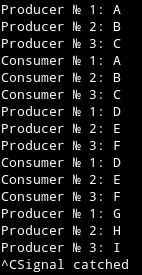
\includegraphics[scale=1]{source/2.png}}
		\caption{Пример работы Программы 1}
	\end{figure}
	\newpage
	
	\section*{Задание 2}
	\addcontentsline{toc}{section}{Задание 2}
	Написать программу, реализующую задачу «Читатели – писатели» по монитору Хоара с четырьмя функциями: Начать\_чтение, Закончить\_чтение, Начать\_запись, Закончить\_запись. В программе всеми процессами разделяется одно единственное значение в разделяемой памяти. Писатели ее только инкрементируют, читатели могут только читать значение.\par
	Для реализации взаимоисключения используются семафоры\par 	
	
	\section*{Программа 2}
	\addcontentsline{toc}{section}{Программа}
	В Листинге 2 показан код программы.\newline
	\begin{lstlisting}	
	#include <stdio.h>
	#include <stdlib.h>
	#include <unistd.h>
	#include <sys/types.h>
	#include <sys/ipc.h>
	#include <sys/sem.h>
	#include <sys/shm.h>
	#include <sys/wait.h>
	#include <sys/stat.h>
	#include <time.h>
	
	#define ACTIVE_WRITER 0
	#define WAITING_WRITER 1
	#define ACTIVE_READER 2
	#define WAITING_READER 3
	
	#define WRITERS 3
	#define READERS 5
	
	int* shared_buffer = NULL;
	
	struct sembuf start_reading[5] =
	{
		{WAITING_READER, 1, 0},
		{ACTIVE_WRITER, 0, 0},
		{WAITING_WRITER, 0, 0}, 
		{ACTIVE_READER, 1, 0},
		{WAITING_READER, -1, 0}
	};
	struct sembuf stop_reading[1] = 
	{
		{ACTIVE_READER, -1, 0}
	};
	
	struct sembuf start_writing[5] =
	{
		{WAITING_WRITER, 1, 0},
		{ACTIVE_READER, 0, 0},
		{ACTIVE_WRITER, 0, 0}, 
		{ACTIVE_WRITER, 1, 0},
		{WAITING_WRITER, -1, 0}
	};
	struct sembuf stop_writing[1] = 
	{
		{ACTIVE_WRITER, -1, 0}
	};
	
	int perms = S_IRWXU | S_IRWXG | S_IRWXO;
	
	void error_check(int fd, char* msg)
	{
		if (fd == -1)
		{
			perror(msg);
			exit(1);
		}
	}
	
	int get_sem() 
	{
		int sem = semget(IPC_PRIVATE, 5, IPC_CREAT | perms);
		error_check(sem, "sem");
		
		int s1 = semctl(sem, ACTIVE_WRITER, SETVAL, 0);
		error_check(s1, "semctl");
		
		int s2 = semctl(sem, ACTIVE_READER, SETVAL, 0);
		error_check(s2, "semctl");
		
		int s3 = semctl(sem, WAITING_WRITER, SETVAL, 0);
		error_check(s3, "semctl");
		
		int s4 = semctl(sem, WAITING_READER, SETVAL, 0);
		error_check(s4, "semctl");
		
		return sem;
	}
	
	int get_shared_memory()
	{
		int shared_memory = shmget(IPC_PRIVATE, sizeof(int), IPC_CREAT | perms);
		error_check(shared_memory, "shmget");
		
		shared_buffer = (int*)shmat(shared_memory, 0, 0);
		if (shared_buffer == (int*)-1) 
		{
			perror("shmat\n");
			exit(1);
		}
		
		*shared_buffer = 0;
		
		return shared_memory;
	}
	
	void writer(int sem, int id) 
	{
		while (1)
		{
			error_check(semop(sem, start_writing, 5), "semop");
			
			*shared_buffer += 1;
			printf("Writer  %d: %d\n", id, *shared_buffer);
			
			error_check(semop(sem, stop_writing, 1), "semop");
			
			sleep(rand() % 5);
		}
	}
	
	void reader(int sem, int id) 
	{
		while (1)
		{
			error_check(semop(sem, start_reading, 5), "semop");
			
			printf("Reader  %d: %d\n", id, *shared_buffer);
			
			error_check(semop(sem, stop_reading, 1), "semop");
			
			sleep(rand() % 5);
		}
	}
	
	void catch_signal(int signalNum)
	{
		printf("Signal catched\n");
	}
	
	int main()
	{
		srand(time(NULL));
		int shared_memory = get_shared_memory();
		int sem = get_sem();
		
		for (int i = 0; i < WRITERS; i++) 
		{
			pid_t pid = fork();
			error_check(pid, "fork");
			
			if (pid == 0) 
			{
				writer(sem, i + 1);
				exit(0);
			}
		}
		
		for (int i = 0; i < READERS; i++) 
		{
			pid_t pid = fork();
			error_check(pid, "fork");
			
			if (pid == 0) 
			{
				reader(sem, i + 1);
				exit(0);
			}
		}
		
		signal(SIGINT, catch_signal);
		
		for (int i = 0; i < (WRITERS + READERS); i++)
		{
			int status;
			wait(&status);
		}
		
		shmctl(shared_memory, IPC_RMID, NULL);
		
		return 0;
	}
	\end{lstlisting}

	\newpage
	Ниже на Рисунке 2 показан пример работы данной программы.
	\begin{figure}[h!]
		\centering{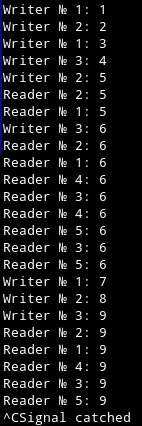
\includegraphics[scale=1]{source/1.png}}
		\caption{Пример работы Программы 2}
	\end{figure}

\end{document}